\documentclass{beamer}
\usepackage{../tut-slides}
\usepackage{../mathoperatorsAuD}

\usepackage{lmodern}
\usepackage{amsmath,amssymb}
\usepackage{stmaryrd}
\usepackage{enumerate}
%\usepackage[inline]{enumitem} 		%customize label
%\newcommand{\labelitemi}{\raisebox{1pt}{\scalebox{.9}{$\blacktriangleright$}}}
%\newcommand{\labelitemii}{$\vartriangleright$}
%\newcommand{\labelitemiii}{--}
\setbeamertemplate{itemize item}{\raisebox{1pt}{\scalebox{.9}{$\blacktriangleright$}}}
\setbeamertemplate{itemize subitem}{$\vartriangleright$}

\usepackage{booktabs}
\usepackage{tabularx}
\usepackage{tabu}
\newcommand*\head{\rowfont{\bfseries}}
\newcommand*{\tw}{\rowfont{\ttfamily}}
\renewcommand{\tabularxcolumn}[1]{>{\hspace{0pt}}m{#1}}
\usepackage{multirow}

\usepackage{cancel}

\usepackage{empheq}
\newcommand*\widefbox[1]{\fbox{\hspace{2em} #1 \hspace{2em}}}

\usepackage{tcolorbox}
\newtcolorbox{mymathbox}[1][]{colback=white, sharp corners, #1}

\usepackage{xcolor}
\usepackage{listings}
\newcommand*{\ttfamilywithbold}{\fontfamily{lmtt}\selectfont}
\lstset{numbers=left, 
	numberstyle=\tiny, 
	breaklines=true,
	backgroundcolor=\color{cdgray!10},
	numbersep=5pt,
	language=C,
	tabsize=2,
	basicstyle=\footnotesize\ttfamilywithbold,
	showstringspaces=false} 

\DeclareMathOperator{\ack}{\mathbf{ack}}
\usepackage{MnSymbol}

\newcommand{\col}[1]{\textcolor{cdpurple}{#1}}
\newcolumntype{R}[1]{>{\centering\arraybackslash}p{#1}}

\begin{document}	
	\title{Algorithmen und Datenstrukturen}
	\subtitle{Übung 5: C \& Pulsierender Speicher}
	\author{Eric Kunze}
	\email{eric.kunze@mailbox.tu-dresden.de}
	\city{TU Dresden}
%	\institute{Lehrstuhl für Grundlagen der Programmierung}
	\titlegraphic{
\includegraphics[width=2cm]{../TUD-white.pdf}}
	\date{27.11.2020}

	\maketitle


%%%%%%%%%%%%%%%%%%%%%%%%%%%%%%%%%%%%%%%%%%%%%%%%%%%%%%%%%%%%%%%%%%%%%%%%%%%%%

\begin{frame} \frametitle{Die Ackermann-Funktion}
	\begin{quote} \small
		''Die Ackermannfunktion ist eine 1926 von Wilhelm Ackermann gefundene, extrem schnell wachsende mathematische Funktion, mit deren Hilfe in der theoretischen Informatik Grenzen von Computer- und Berechnungsmodellen aufgezeigt werden können.`` \\
		\upshape \tiny Quelle: \url{https://de.wikipedia.org/wiki/Ackermannfunktion}
	\end{quote}

	\textbf{Definition von  $\ack : \N \times \N \to \N$}
	\begin{align*}
		\ack(0,y) &= y + 1 &(y \ge 0) \\
		\ack(x,0) &= \ack(x-1,1) &(x > 0)\\
		\ack(x,y) &= \ack(x-1,\ack(x,y-1)) &(x,y > 0)
	\end{align*}
\end{frame}

\begin{frame} \frametitle{Die Ackermann-Funktion}
\textbf{Definition von  $\ack : \N \times \N \to \N$}
	\begin{align*}
	\ack(0,y) &= y + 1 &(y \ge 0) \\
	\ack(x,0) &= \ack(x-1,1) &(x > 0)\\
	\ack(x,y) &= \ack(x-1,\ack(x,y-1)) &(x,y > 0)
	\end{align*}
	
	\textbf{einige Werte}
	
	\begin{small}
		\begin{tabular}{c||ccccccc}
			$x \ \backslash \ y$ & $0$ & $1$ & $2$ & $3$ & $4$ & $\dots$ & $m$ \\ \hline\hline
			$0$ & $1$ & $2$ & $3$ & $4$ & $5$ & $\dots$ & $m+1$ \\
			$1$ & $2$ & $3$ & $4$ & $5$ & $6$ & $\dots$ & $m+2$ \\
			$2$ & $3$ & $5$ & $7$ & $9$ & $11$ & $\dots$ & $2m+3$ \\
			$3$ & $5$ & $13$ & $29$ & $61$ & $125$ & $\dots$ & $8*2^m-3$ \\
			$4$ & $13$ & $65533$ & $2^{65536} -3$ & $\dots$ & $\dots$ & $\dots$ & $\underbrace{2^{2^{{\udots}^2}} }_{m+3}- 3$ 
		\end{tabular}
	\end{small}	
\end{frame}

\begin{frame}[fragile] \frametitle{Aufgabe 1}
	\footnotesize
\begin{lstlisting}
#include <stdio.h>
int ack(int x, int y){
	int a;
	if ((x == 0) && (y >= 0))       return y + 1;
	else if ((x > 0) && (y == 0))   return ack(x-1, 1);
	else if ((x > 0) && (y > 0)){
		a = ack(x, y-1);
		return ack(x-1, a);   }
}
int main() {
	int x = 0, y = 0, a;
	printf("\nAckermannfunktion\n");
	printf("x = ");   scanf("%d", &x);
	printf("y = ");   scanf("%d", &y);
	a = ack(x,y);
	printf("ack(%i,%i)=%i.\n", x, y, a);
	return 0;
}
\end{lstlisting}
\end{frame}

%%%%%%%%%%%%%%%%%%%%%%%%%%%%%%%%%%%%%%%%%%%%%%%%%%%%%%%%%%%%%%%%%%%%%%%%%%%%%%%%%%%
\begin{frame} \frametitle{Aufgabe 2}
	\centering
	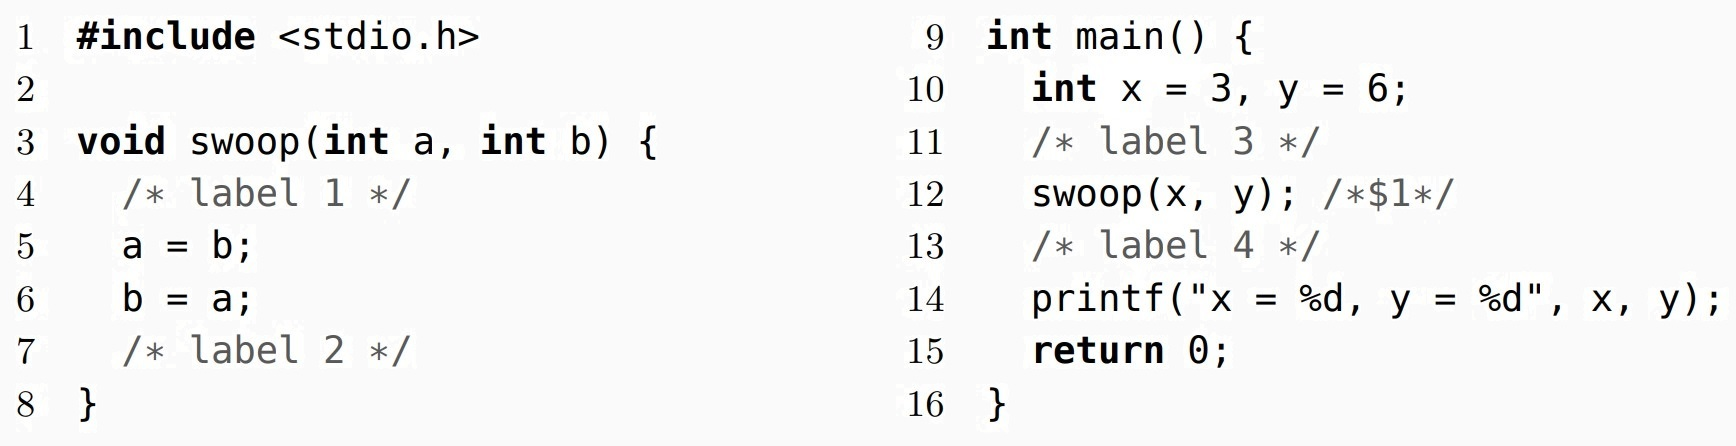
\includegraphics[width=\textwidth]{./tut05_aufgabe2.jpg}
\end{frame}

\begin{frame} \frametitle{Aufgabe 2 --- Teil (a)}
	\centering
	\def\arraystretch{0.9}
	\begin{tabular}{|p{1.5cm}|r||R{0.4cm}|R{0.4cm}|R{0.4cm}|R{0.4cm}|}
		\hline
		Label & RM & 1 & 2 & 3 & 4 \\ 
		\hline \hline
		\multirow{2}{*}{label3} & \multirow{2}{*}{---} & x & y &   & \\ 
		&                      & 3 & 6 &   & \\ \hline
		\multirow{2}{*}{label1} & \multirow{2}{*}{1}   &   &   & a & b \\      
		&                      &   &   & 3 & 6 \\ \hline
		\multirow{2}{*}{label2} & \multirow{2}{*}{1}   &   &   & a & b \\    
		&                      &   &   & 6 & 6 \\ \hline  
		\multirow{2}{*}{label4} & \multirow{2}{*}{---} & x & y &   &   \\ 
		&                      & 3 & 6 &   &   \\ \hline
	\end{tabular}
\end{frame}

\begin{frame}[fragile] \frametitle{Aufgabe 2 --- Teil (b)}
\begin{lstlisting}
#include <stdio.h>
void swap(int *x, int *y){ 
	int tmp;
	tmp = *x; 
	*x = *y;
	*y = tmp;
}
int main() {
	int x = 4, y = 6;
	printf("x = %d, y = %d \n", x, y);
	swap(&x, &y);
	printf("x = %d, y = %d \n", x, y);
	return 0;
}
\end{lstlisting}
\end{frame}

%%%%%%%%%%%%%%%%%%%%%%%%%%%%%%%%%%%%%%%%%%%%%%%%%%%%%%%%%%%%%%%%%%%%%%%%%%%%%%%%%%%
\begin{frame} \frametitle{Aufgabe 3}
	\centering
	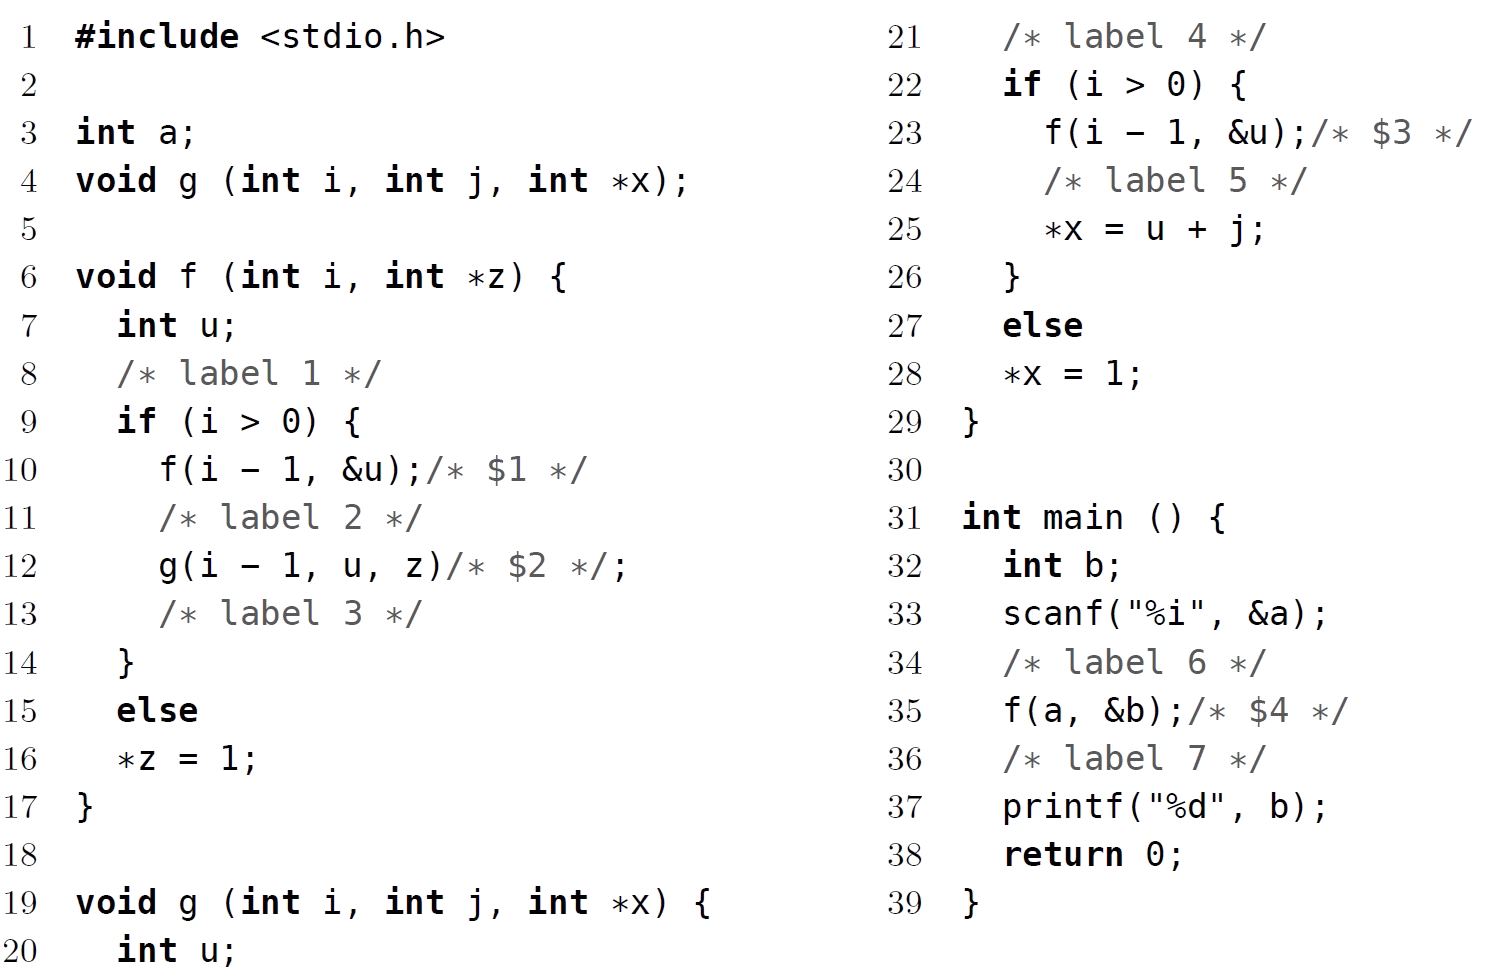
\includegraphics[width=\textwidth]{./tut05_aufgabe3.png}
\end{frame}

\begin{frame} \frametitle{Aufgabe 3 --- Teil (a)}
	\textbf{Gültigkeitsbereiche}

	\centering
	\begin{tabular}{|l|c|}
		\hline
		Objektname & Gültigkeitsbereich \\ \hline \hline
		\texttt{a} & 3 -- 39 \\ \hline
		\texttt{g} & 4 -- 39 \\ \hline
		\texttt{i,j,x} in \texttt{g} & 19 -- 29 \\ \hline
		\texttt{u} in \texttt{g} & 20 -- 29 \\ \hline
		\texttt{f} & 6 -- 39 \\ \hline
		\texttt{i,z} in \texttt{f} & 6 -- 17 \\ \hline
		\texttt{u} in \texttt{f} & 7 -- 17 \\ \hline
		\texttt{main} & 31 -- 39 \\ \hline
		\texttt{b} in \texttt{main} & 32 -- 39 \\ \hline
	\end{tabular}
\end{frame}

\begin{frame} \frametitle{Aufgabe 3 --- Teil (b)}
	\tiny \centering
	\def\arraystretch{0.9}
	\begin{tabular}{|p{1cm}|r||R{0.25cm}|R{0.25cm}|R{0.25cm}|R{0.25cm}|R{0.25cm}|R{0.25cm}|R{0.25cm}|R{0.25cm}|R{0.25cm}|R{0.25cm}|R{0.25cm}|R{0.25cm}|}
		\hline
		Label & RM & 1 & 2 & 3 & 4 & 5 & 6 & 7 & 8 & 9 & 10 & 11 & 12 \\ 
		\hline \hline
		label1 & 4     & a &  & i       & z   & u &   &   &   &   &   &   & \\ 
	           &       & 2 &  & 2       & 2   & ? &   &   &   &   &   &   & \\ \hline
		label1 & 1:4   & a &  &         &     &   & i & z & u &   &   &   & \\ 
		       &       & 2 &  &         &     &   & 1 & \col{5} & ? &   &   &   & \\ \hline
		label1 & 1:1:4 & a &  &         &     &   &   &   &   & i & z & u & \\ 
		       &       & 2 &  &         &     &   &   &   &   & 0 & \col{8} & ? & \\ \hline
		label2 & 1:4   & a &  &         &     &   & i & z & u &   &   &   & \\ 
		       &       & 2 &  &         &     &   & 1 & \col{5} & 1 &   &   &   &\\ \hline
		label4 & 2:1:4 & a &  &         &     &   &   &   &   & i & j & x & u \\ 
		       &       & 2 &  &         &     &   &   &   &   & 0 & 1 & \col{5} & ? \\ \hline
		label3 & 1:4   & a &  &         &     &   & i & z & u &   &   &   & \\ 
		       &       & 2 &  &         &     & 1 & 1 & \col{5} & 1 &   &   &   & \\ \hline
	\end{tabular}

	\begin{tabular}{|p{1cm}|r||R{0.25cm}|R{0.25cm}|R{0.25cm}|R{0.25cm}|R{0.25cm}|R{0.25cm}|R{0.25cm}|R{0.25cm}|R{0.25cm}|R{0.25cm}|R{0.25cm}|R{0.25cm}|}
		\hline
		Label & RM & 1 & 2 & 3 & 4 & 5 & 6 & 7 & 8 & 9 & 10 & 11 & 12 \\ 
		\hline \hline
		label2 & 4          & a &   & i       & z   & u &   &   &   &   &   &   & \\ 
		       &            & 2 &   & 2       & 2   & 1 &   &   &   &   &   &   & \\ \hline
		label4 & 2:4        & a &   &         &     &   & i & j & x & u &   &   & \\ 
		       &            & 2 &   &         &     &   & 1 & 1 & 2 & ? &   &   & \\ \hline
		label1 & 3:2:4      & a &   &         &     &   &   &   &   &   & i & z & u \\ 
		       &            & 2 &   &         &     &   &   &   &   &   & 0 & \col{9} & ? \\ \hline
		label5 & 2:4        & a &   &         &     &   & i & j & x & u &   &   & \\ 
		       &            & 2 &   &         &     &   & 1 & 1 & 2 & 1 &   &   &\\ \hline
		label3 &     4      & a &   & i       & z   & u &   &   &   &   &   &   &   \\ 
		       &            & 2 & 2 & 2       & 2   & 1 &   &   &   &   &   &   &   \\ \hline
		label7 & $\epsilon$ & a & b &         &     &   &   &   &   &   &   &   & \\ 
		       &            & 2 & 2 &         &     &   &   &   &   &   &   &   & \\ \hline
	\end{tabular}
\end{frame}



%%%%%%%%%%%%%%%%%%%%%%%%%%%%%%%%%%%%%%%%%%%%%%%%%%%%%%%%%%%%%%%%%%%%%%%%%%%%%%%%%%%

\end{document}